\chapter{State of Art}
\section{Smart Home Research}
\subsection{Overview}
The smart home system we discussed about, that is also described as automated home, integrated home systems or intelligent building\cite{smart_home_concept}, has drawn more and more industry developers' and researchers' attention over the decades, research groups such as Siemens, IBM, Cisco, Microsoft\cite{smart_home_research} has already contributed in this domain. A great number of Smart Home application, network protocols as well as gateways\cite{smart_home_for_gateway} haven come into world and been applied to benefit their customers.

With the development of Smart Home technology, nowadays' Smart Home is not only  in charge of monitoring and controlling lighting and heating inside the building, but also capable of connecting almost every electronic devices, inhabitant action prediction as well as making scheduler decisions. Functionalities provided by intelligent home are not just limited to turn device on and off, record and report senor data, but include self-adjusting the inner building environment, supporting various predefined pattern, such as energy saving pattern, especially the concept of Smart Home for elderly\cite{smart_home_for_old}, which perfectly combines modern remote control and monitoring technologies, with senior-friendly and patient-concerning housing, is welcomed by the market. 

Three categories of Smart Home will be introduced in the following as best practice examples, they are Smart Home optimized for energy services , Smart Health Home and Agent-based Smart Home.
 
\subsection{Smart Home Optimized for Energy Services}
This type of Smart Home put its main goal in the energy saving and monitoring domain, which helps householder to make wiser decisions in under the energy crisis background. 

The key component in this Smart Home is decision-support tool\cite{smart_home_for_energy}, that applies a scheduling algorithm which offers house owner suggestion based on various parameters such as distributed energy resources(DER), with the prospect of energy and resource saving.

\subsubsection{Decision Support Tool}

 \begin{figure}[!htbp]
	\centering
	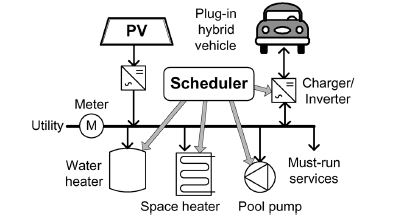
\includegraphics[width=1.0\textwidth]{scheduler.jpg}
		\caption{DER Scheduler in Smart Home optimized for energy\cite{smart_home_for_energy}}
	\label{fig:smart-home-scheduler}
\end{figure}

The decision support tool used in paper\cite{smart_home_for_energy} consists of two components, they are energy service model which describes the energy service request and distributed energy resource scheduling algorithm, as described in figure~\ref{fig:smart-home-scheduler} . To be more specifically, energy service model presents  the demand for one particular energy resource. For instance the demand aimed at hot water means, the hourly consumption of heated water or the energy that is hourly needed by water heater.  According to \cite{smart_home_for_energy}, the heat content of water is also defined as "energy equivalent" and therefore the energy service model is applied to increase "monetary benefit"  from every "energy equivalent" unit.

Meanwhile the DER scheduler algorithm helps householder by reducing the unnecessary consumption of energy. This algorithm is in nature one mathematical optimization problem defined by\cite{smart_home_for_energy}.
\begin{center}
 $ \sum_{t=1}^{T}\sum_{i=1}^{S}[\lambda_{ES,i}(t)\cdot {U_{ES,i}}(t,x)]-Cost$
\end{center}

The purpose of DER scheduler, presented as \emph{x} is to maximize that above introduced fitness function, where \emph{S} represents all number of services offered by Smart Home, \emph{T} stands for the whole simulation time, $\lambda_{ES,i}$ and $ U_{ES,i}$ describe the desired monetary benefit for "energy equivalent" and energy demand of the \emph{i}th service respectively. \emph{Cost} means the total electricity consumption. Also in paper\cite{smart_home_for_energy} the choice of DER algorithm is well discussed.


\subsection{Smart Health Home}
Another suitable application domain for Smart Home is the Smart Health Home, which describes the intelligent housing that takes care of patients at home or elder resident.

The charming features of this Smart Home system are the combination telemedical system with communication technologies\cite and customizing services such as, teleconsulting, telediagnosis, real time imaging as well as distance medical education\cite{smart_home_for_health}, which together improve the living condition of householder and at the same time build a caring system that takes care of residents' need. Nine best practice examples are provided and evaluated in paper\cite{smart_home_for_old}, they provide a guideline for  the design of Smart  Home system and summarizes precious experience. 
 \begin{figure}[!htbp]
	\centering
	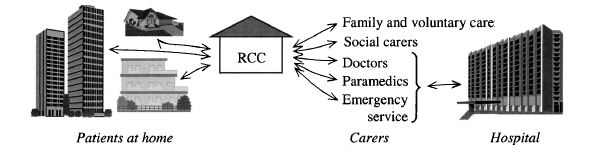
\includegraphics[width=1.0\textwidth]{rcc.jpg}
		\caption{Overview of Smart Health Home structure\cite{smart_home_for_health} (RCC: Remote Control Center)}
	\label{fig:rcc}
\end{figure}
\subsection{Agent-based Smart Home}
Agent-based Smart Home aims to build an intelligent home that can based on machine learning, artificial intelligence technology and mobile computing predict behaviors taken by householder, make appropriate decisions. The achieved prediction can help residents to experience more comfortable and convenience living condition.  MavHome ( Managing An Intelligent Versatile Home)\cite{smart_home_agent} builds the best example. 

\subsubsection{MavHome architecture}
 \begin{figure}[!htbp]
	\centering
	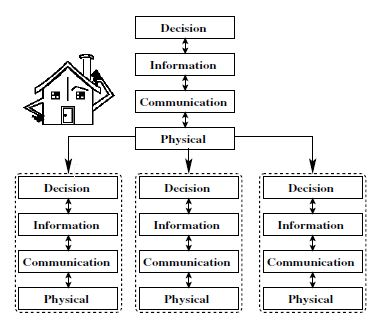
\includegraphics[width=0.8\textwidth]{smart-home-agent.jpg}
		\caption{MavHome agent architecture\cite{smart_home_agent}}
	\label{fig:smart-home-agent}

\end{figure}
As shown in figure~\ref{fig:smart-home-agent}, agents which are employed by MavHome consist of four different layers. From bottom to top:
\begin{itemize}
\item \emph{Physical layer}, where hardwares that together build Smart Home system are deployed. Moreover, underlaying agents can also act as physical layer for other agents.
\item \emph{Communication layer}, this layer provides communication services for agent by using functionalities offered by physical layer.
\item \emph{Information layer}, as higher layer of Smart Home system,  the responsibilities for this layers are gathering and maintaining information which is used by decision layer.
\item \emph{Decision layer}, in this layer agents make decision as well as learn resident's preference and correct the unwanted system behavior.
\end{itemize}
\subsubsection{Prediction algorithm}
Prediction algorithm is the core component of MavHome project. Several Strategies are presented on the first IEEE international conference on pervasive computes and communication, they are SHIP algorithm that is based on sequence matching, compression-based prediction algorithm ALZ and Task-based Markov model\cite{smart_home_agent}.

\subsection{Conclusion}
Also described above, Smart Home is the representative application which is based on industrial automation, remote control, management and coordination system. Despite the decision making algorithms and application level components from above mentioned smart buildings are different from the other, but they all are integrated upon or connected with housing devices. The management and cooperation with those devices must take place under a secure system environment. None of householders are willing to be monitored by a strange third party using his own camera or to expose their daily life related information to public. Therefore one common request for the design of such intelligent building is to ensure the system security.

Based on the fact, that home devices applied by Smart Home are manufactured by various vendors,  Smart Home designers also must take it into account, that how to realize the system interoperability. Considered those two requirements, the idea of this thesis applying OPC UA standards with smart card technology came into world. 

\section{OPC UA Application and Security policy }

\subsection{OPC UA applications}
OPC UA ,as explained in former paragraphs,  is understood as a platform independent, well designed, secure concerned, IEC standard compliant, promising industry standards set, which provides a service oriented architecture, that is being widely applied in industry application such as critical control system and industrial automation. Application examples are given in following paragraphs, each of which has different focus. To be more specifically, the charming characteristics demonstrated are: secure consideration, real time data exchange and management, scalability. 

\subsubsection{OPC UA and ICS}
With develop of industrial automation, Industrial control system (ICS) has became a hot topic, but most manufactures put the much more effort in designing automation and manufacturing process and neglect  the communication security. As a consequence, Cyber security of ICS now is drawing more and more attentions from industry. OPC UA offers manufactures who are applying ICS system not only object oriented modeling rules, which can be extremely helpful for developers that design domain specific model and manufacturing process, but also provides them a reliable and robust security model\cite{opc_ics}, that has various secure arrangements in each communication protocol stack layer.


\subsubsection{OPC UA and  Smart Grid}
Smart Grid is now concerned as the future of electricity energy industry and therefor how to achieve an intelligent electricity distribution as well as behavior coordination between customs and suppliers is a hot topic\cite{opc_grid}. Electricity industry is search out for a standardized communication technology to solve aforementioned issue.
OPC UA standards that include \emph{alarm and even} model, \emph{data access} model as well as  \emph{historical data access} model, is without doubt become one the of best candidates. With the help of all these models,  the secure real-time communication and stockholders' coordination are guaranteed.

\subsubsection{Nano OPC UA }
After from those enterprise level systems, OPC UA is also suitable for lower level field devices, such as field sensor and other resource limited facilities. Recently a German company Lemgo even designed a nano embedded OPC UA server\cite{opc_lemgo}, which provides the core OPC UA server service set. adopts TCP binary communication protocol  and  is implemented on a chip device.

\subsection{OPC UA secure policies}
At the design beginning, the OPC foundation has taken the construction of secure and robust communication protocol as the center and therefore developed a enhanced consistent security model which has clear and definite objectives in each layer of OPC UA transport and communication stack. In present day, OPC UA  offers secure messaging mechanisms by applying WS Security with Simple Object Access Protocol (SOAP)  and alternatively SSL based Hypertext transfer Protocol Secure (HTTPS) messaging\cite{opc_secure_1}. Besides secure messaging protocols,  authentication mechanisms based on username-password or X.509 certificates are introduced, in order to process mutual authentication among OPC UA applications from different logic levels and hardware devices.

OPC foundation uses the term secure policies\cite{O2} to describe the 
user authentication, user authorization and application authentication mechanisms proposed by one OPC UA server profile. In this server profile, both secure related requirements and other server functionalities are described. One server is capable of maintaining several profiles in order to provides services to different clients, who might have various demands for security. Meanwhile one client can also accept a list of profiles, each of them is assigned by one server with particular security objectives. 

\subsection{OPC UA design consideration}
Along with core services set including data read and write services, notification service etc., OPC UA server also provides \emph{discover service}\cite{O4}, which provides OPC UA clients mechanism to require server secure policy, and \emph{secure channel service} set\cite{O4}, that is used to create and management secure channel with acknowledgment such as key deviation algorithm and encryption algorithm achieved from secure policy. 

Also OPC UA specifications provide guide lines for a secure system design\cite{O4}.
\begin{itemize}
\item \emph{appropriate timeout} Timeout mechanism is widely employed in systems that adopt client server architecture. With reasonable configured timeout property, both client and server can avoid unnecessary resource consumption by long time waiting response from the other, which could be caused by unexpected physical device failure or intentionally server denial of service attack initiated by third party and etc. 
\item \emph{rate control} Rate control is considered as one of the most practical approach to prevent denial of service attack. Under rate control mechanism, each client has limited chance over a period to build communication channel, reconstruct this channel, require information from server or send data to sever. Alternatively server can also ban or block the client for a period of time, who is recently trying to flood messages. 
\item \emph{random number generation} The generation of random number is required by most encryption, authentication and authorization algorithms. Therefore a secure system must support robust random number generation.
\item \emph{strict message processing}, which means the exchanged message between two communication partners must be compliant with predefined message format. Any ill-formed messages must be ignored, which in turn helps to avoid stack overflow attack and enhances system security
\item \emph{historical data management}, this strategy ensures the system traceability and records any behaviors taking place in system. And the recorded data can be used for forensic research, when security related issues happens.
\end{itemize}
\subsection{Conclusion}
Above pictured OPC UA standards' features and characteristics prove the feasibility of applying OPC UA as communication protocol for Smart Home proposed in this thesis.

\section{Smart Card Security}

\section{Secure Android Design}